\documentclass[twocolumn]{rbef}
\usepackage{subfigure}
\usepackage{epstopdf}
\usepackage{cite}
\usepackage{float}
\usepackage{amsthm, wasysym}
\usepackage{thmtools}
% bm removed for TeX Live 2013 compatibility (use \boldsymbol instead)
% siunitx removed for TeX Live 2013 compatibility
\usepackage[T1]{fontenc}

\titulocabecalho{Problema de Störmer e o cinturão de Van Allen}
\autorcabecalho{Cunha e Schmidt}

\newcommand{\PR}[1]{\ensuremath{\left[#1\right]}}
\newcommand{\PC}[1]{\ensuremath{\left(#1\right)}}
\newcommand{\chav}[1]{\ensuremath{\left\{#1\right\}}}

\numeracao{xxxx}
\volume{xx}
\numero{xx}
\ano{20xx}
\doi{http://dx.doi.org/xxxx}
\tipodeartigo{Artigos Gerais}

\author[]{Pedro H. S. Cunha$^{1^*}$, Alexandre G. M. Schmidt$^{1}$}
\affil[]{$^1$ Instituto de Ciências Exatas, Universidade Federal Fluminense, Volta Redonda, RJ, Brasil.
\thanks{\href{emailto:henrique.pedrouff@gmail.com}{henrique.pedrouff@gmail.com}}}

\titulo{Problema de Störmer: um estudo computacional sobre a formação do cinturão de radiação de Van Allen}
\subtitulo{Störmer problem: a computational study on the formation of the Van Allen radiation belt}

\begin{document}

\begin{primeirapagina}

\begin{abstract}
Neste trabalho, apresentamos o problema de Störmer no contexto da mecânica clássica: o movimento de partículas carregadas não relativísticas sob a ação do campo magnético dipolar da Terra. A partir da formulação lagrangiana em coordenadas cilíndricas, obtemos as equações de movimento e identificamos as constantes de movimento do sistema. O sistema resultante é não integrável, e recorremos ao método simplético de Störmer-Verlet de segunda ordem para integrar numericamente as equações de movimento. Três casos são analisados: o caso equatorial, em que a partícula permanece restrita ao plano $Z = 0$; o caso tridimensional completo; e o caso vinculado a uma superfície esférica. No caso equatorial, mostramos que o potencial efetivo possui um mínimo e um máximo locais, e que partículas com energia abaixo do máximo ficam confinadas em órbitas oscilatórias. No caso tridimensional, a dinâmica apresenta sensibilidade às condições iniciais e trajetórias que reproduzem a estrutura toroidal do cinturão de radiação de Van Allen. No caso esférico, o sistema torna-se integrável e admite solução analítica em funções elípticas de Jacobi, permitindo validar a precisão do integrador numérico.
\palavraschave{Problema de Störmer, cinturão de Van Allen, integração simplética, mecânica clássica.}
\end{abstract}

\begin{otherlanguage}{english}
\begin{abstract}
We present the Störmer problem in the framework of classical mechanics: the motion of non-relativistic charged particles under the Earth's dipolar magnetic field. Starting from the Lagrangian formulation in cylindrical coordinates, we derive the equations of motion and identify the conserved quantities. The resulting system is non-integrable, and we employ the second-order symplectic Störmer-Verlet method to numerically integrate the equations of motion. Three cases are analyzed: the equatorial case, where the particle is restricted to the $Z = 0$ plane; the full three-dimensional case; and the case where the particle is constrained to a spherical surface. In the equatorial case, we show that the effective potential has a local minimum and maximum, and that particles with energy below the maximum are confined to oscillatory orbits. In the three-dimensional case, the dynamics exhibits sensitivity to initial conditions and trajectories that reproduce the toroidal structure of the Van Allen radiation belt. In the spherical case, the system becomes integrable and admits an analytical solution in Jacobi elliptic functions, which we use to validate the numerical integrator.
\keywords{Störmer problem, Van Allen radiation belt, symplectic integration, classical mechanics.}
\end{abstract}
\end{otherlanguage}

\end{primeirapagina}
\saythanks

\section{Introdução}

\subsection{As auroras e o problema de Störmer}

As auroras polares são registradas em relatos desde a Antiguidade, porém uma explicação física para o fenômeno só surgiu no final do século XIX. Em 1896, o físico norueguês Kristian Birkeland propôs que as auroras seriam causadas por feixes de partículas carregadas emitidas pelo Sol e deflectidas pelo campo magnético da Terra em direção aos polos \cite{Birkeland}. Para testar essa hipótese, Birkeland construiu um dispositivo experimental conhecido como \textit{terrella}: uma esfera magnetizada, com um eletroímã interno, colocada dentro de uma câmara de vácuo. Ao disparar raios catódicos contra a terrella, Birkeland observou que os elétrons se concentravam em regiões anulares ao redor dos polos magnéticos da esfera, reproduzindo em laboratório o padrão geográfico das auroras \cite{Birkeland}.

Quem se dedicou a tratar o problema de forma matemática rigorosa foi Carl Störmer (1874--1957), matemático e físico norueguês contemporâneo de Birkeland. Störmer formulou as equações de movimento de partículas carregadas sob a ação de um campo magnético dipolar e dedicou-se, ao longo de décadas, a calcular numericamente milhares de trajetórias de partículas, identificando padrões de confinamento e espalhamento que dependiam das condições iniciais \cite{Stormer, Stormer2}. Os cálculos eram feitos à mão, com o auxílio de assistentes, e os resultados foram compilados em seu livro \textit{The Polar Aurora}, publicado em 1955 \cite{Stormer3}. Os métodos numéricos que Störmer desenvolveu para integrar as equações de movimento, baseados em fórmulas de diferenças finitas com múltiplos passos, são, de certa forma, os precursores dos integradores simpléticos modernos, como veremos na Seção 3.

Em paralelo ao trabalho de Störmer, o estudo dos raios cósmicos trouxe evidências independentes da influência do campo geomagnético sobre partículas carregadas. No início da década de 1930, Clay e Berlage \cite{Clay} e, logo em seguida, Compton \cite{Compton} observaram que a intensidade dos raios cósmicos que atingem a superfície terrestre depende da latitude geográfica: a intensidade é menor próxima ao equador e maior em latitudes elevadas. Esse \textit{efeito de latitude} tem uma explicação direta no contexto do problema de Störmer. O campo magnético dipolar é mais intenso na região equatorial e deflete as partículas de menor energia, que não conseguem penetrar até a superfície. Em latitudes altas, onde as linhas de campo convergem e se aproximam da vertical, as partículas encontram menos resistência magnética e atingem a atmosfera com maior facilidade. A análise quantitativa de Störmer já previa esse comportamento, e a confirmação experimental do efeito de latitude fortaleceu a validade do modelo dipolar.

\subsection{A descoberta dos cinturões de Van Allen}

A confirmação mais direta das previsões de Störmer veio em 1958, no contexto da corrida espacial. O satélite Explorer 1, lançado em janeiro daquele ano, carregava um detector Geiger projetado pelo físico James Van Allen e sua equipe na Universidade de Iowa. Os dados transmitidos pelo satélite revelaram algo inesperado: em determinadas altitudes, o contador Geiger saturava, indicando níveis de radiação muito acima do previsto. A princípio, houve dúvida sobre se o instrumento havia falhado. Medições complementares do satélite Explorer 3, lançado em março de 1958, confirmaram que a saturação era real \cite{VanAllen}. O que os detectores registravam era a presença de grandes quantidades de prótons e elétrons aprisionados pelo campo magnético terrestre, concentrados em duas regiões toroidais ao redor da Terra, exatamente o tipo de confinamento que Störmer havia previsto teoricamente décadas antes.

Essas regiões receberam o nome de cinturões de radiação de Van Allen. O cinturão interno, situado entre aproximadamente 1.000 e 6.000 km de altitude, é composto predominantemente por prótons de alta energia. O cinturão externo, entre cerca de 13.000 e 60.000 km, contém majoritariamente elétrons. A existência desses cinturões tem consequências práticas: satélites e sondas que atravessam ou orbitam nessas regiões ficam expostos a níveis elevados de radiação, que podem danificar componentes eletrônicos e representar riscos para astronautas \cite{atlantico, ESA, Stassinopoulos}. A Anomalia Magnética do Atlântico Sul, uma região onde o cinturão interno se aproxima da superfície terrestre devido a irregularidades no campo geomagnético, é um exemplo concreto desse problema: satélites em órbita baixa sofrem maior incidência de falhas eletrônicas ao passarem sobre essa região \cite{atlantico}.

\subsection{Contexto e objetivos deste trabalho}

Do ponto de vista da mecânica analítica, o problema de Störmer é um sistema hamiltoniano com dois graus de liberdade efetivos (as coordenadas $\rho$ e $Z$ no plano meridional, após a eliminação da coordenada azimutal $\phi$ pela conservação do momento canônico). Apesar de possuir duas constantes de movimento, a energia e o momento angular canônico, o sistema não é integrável no sentido de Liouville \cite{ruidilao, Saletan}. Esse fato, demonstrado rigorosamente por Dilão e Alves-Pires, significa que não existe uma terceira constante de movimento independente que permita reduzir o sistema a quadraturas. A consequência prática é que as equações de movimento só podem ser resolvidas numericamente, e que certas trajetórias apresentam sensibilidade exponencial às condições iniciais, ou seja, comportamento caótico.

O objetivo deste artigo é apresentar o problema de Störmer com a formulação matemática completa e a implementação computacional, em um nível adequado para estudantes de graduação em física. O problema reúne, num mesmo contexto físico, a formulação lagrangiana e hamiltoniana, a identificação de constantes de movimento por simetria, a análise de potencial efetivo e a integração numérica de sistemas dinâmicos. O método numérico escolhido, o integrador de Störmer-Verlet, tem, além disso, uma conexão histórica com o próprio problema: como discutiremos na Seção 3, Störmer foi um dos primeiros a usar esquemas de diferenças finitas desse tipo, precisamente para calcular as trajetórias de partículas no campo dipolar.

Na Seção 2, derivamos as equações de movimento a partir da força de Lorentz e da formulação lagrangiana, e introduzimos as grandezas adimensionais utilizadas na simulação. Na Seção 3, apresentamos o método de Störmer-Verlet, sua origem histórica e suas propriedades como integrador simplético. Na Seção 4, discutimos os resultados numéricos para o caso equatorial, o caso tridimensional e o caso vinculado à esfera. Na Seção 5, apresentamos as conclusões.

\section{Formulação do problema}

\subsection{Equações de movimento}

Considere uma partícula não relativística de massa $m$ e carga $q$ movendo-se sob a ação de um campo magnético $\boldsymbol{B}$. A equação de movimento, dada pela força de Lorentz, é

\begin{equation}\label{lorentz}
    m\boldsymbol{\ddot{r}} = q\left(\boldsymbol{\dot{r}} \times \boldsymbol{B}\right).
\end{equation}

Modelamos o campo magnético terrestre como o campo gerado por um dipolo magnético $\boldsymbol{\mu}_z = \mu \boldsymbol{e}_z$ posicionado no centro da Terra, com o eixo do dipolo alinhado ao eixo de rotação. O potencial vetor associado a esse dipolo é

\begin{equation}\label{potencialVetor}
    \boldsymbol{A} = \dfrac{\mu_0}{4\pi}\dfrac{\boldsymbol{\mu}_z \times \boldsymbol{e}_r}{r^2} = M_z\dfrac{1}{r^3}\left(-y\boldsymbol{e}_x + x\boldsymbol{e}_y\right),
\end{equation}

\noindent onde $M_z = \mu_0 \mu / (4\pi)$ é o momento de dipolo magnético efetivo e $r = \sqrt{x^2 + y^2 + z^2}$. O campo magnético é então obtido por $\boldsymbol{B} = \nabla \times \boldsymbol{A}$.

Substituindo o campo resultante na equação (\ref{lorentz}), obtemos as equações de movimento em coordenadas cartesianas:

\begin{equation}\label{eqCartesianas}
    \begin{cases}
    \ddot{x} = 3\alpha\dfrac{z}{r^5}\left(\dot{y}z - \dot{z}y\right) - \alpha\dot{y}\dfrac{1}{r^3}\\[8pt]
    \ddot{y} = -3\alpha\dfrac{z}{r^5}\left(\dot{x}z - \dot{z}x\right) + \alpha\dot{x}\dfrac{1}{r^3}\\[8pt]
    \ddot{z} = 3\alpha\dfrac{z}{r^5}\left(\dot{x}y - \dot{y}x\right)
    \end{cases}
\end{equation}

\noindent onde a constante $\alpha = qM_z/m$ condensa as propriedades da partícula e do dipolo. Para o campo magnético terrestre, o momento de dipolo efetivo vale $M_z \approx 8{,}2 \times 10^{15}\,\text{T}\cdot\text{m}^3$, e os valores de $\alpha$ para elétrons e prótons são

\begin{equation}
    \alpha = \begin{cases}
                -1{,}44 \times 10^{27}\,\text{m}^3/\text{s} & \textrm{(elétrons)}\\[4pt]
                7{,}87 \times 10^{23}\,\text{m}^3/\text{s} & \textrm{(prótons)}
            \end{cases}
\end{equation}

\subsection{Adimensionalização}

Para trabalhar com grandezas de ordem unitária, realizamos uma mudança de escala usando o raio terrestre $r_0 = 6\,378\,136\,\text{m}$ como unidade de comprimento. Definimos as coordenadas adimensionais $X = x/r_0$, $Y = y/r_0$ e $Z = z/r_0$, de modo que $R = \sqrt{X^2 + Y^2 + Z^2}$ é a distância em unidades de raios terrestres. As equações de movimento tornam-se

\begin{equation}\label{eqAdimensional}
    \begin{cases}
    \ddot{X} = 3\alpha_1\dfrac{Z}{R^5}\left(\dot{Y}Z - \dot{Z}Y\right) - \alpha_1\dot{Y}\dfrac{1}{R^3}\\[8pt]
    \ddot{Y} = -3\alpha_1\dfrac{Z}{R^5}\left(\dot{X}Z - \dot{Z}X\right) + \alpha_1\dot{X}\dfrac{1}{R^3}\\[8pt]
    \ddot{Z} = 3\alpha_1\dfrac{Z}{R^5}\left(\dot{X}Y - \dot{Y}X\right)
    \end{cases}
\end{equation}

\noindent com a constante adimensionalizada

\begin{equation}
    \alpha_1 = \dfrac{\alpha}{r_0^3} = \begin{cases}
                -5{,}57 \times 10^{6}\,\text{s}^{-1} & \textrm{(elétrons)}\\[4pt]
                3{,}04 \times 10^{3}\,\text{s}^{-1} & \textrm{(prótons)}
            \end{cases}
\end{equation}

Observe que a diferença de três ordens de grandeza entre $\alpha_1$ para elétrons e prótons reflete a diferença de massa entre as duas partículas, e implica que os elétrons realizam oscilações muito mais rápidas.

\subsection{Formulação lagrangiana e hamiltoniana}

O problema possui simetria cilíndrica em torno do eixo do dipolo. É conveniente, portanto, utilizar coordenadas cilíndricas $(\rho, \phi, Z)$, onde $\rho = \sqrt{X^2 + Y^2}$. Nessas coordenadas, a lagrangiana do sistema é

\begin{equation}\label{lagrangiana}
    L = \dfrac{m}{2}\left(\dot{\rho}^2 + \rho^2\dot{\phi}^2 + \dot{Z}^2\right) + m\alpha_1\dfrac{\rho^2}{R^3}\dot{\phi},
\end{equation}

\noindent onde $R = \sqrt{\rho^2 + Z^2}$. O último termo é a contribuição do potencial vetor, e acopla o grau de liberdade azimutal ao campo magnético. A derivação completa da lagrangiana a partir do formalismo de partícula em campo eletromagnético pode ser encontrada em \cite{Goldstein, Taylor}.

O sistema possui três momentos canônicos: $p_\rho = m\dot{\rho}$, $p_Z = m\dot{Z}$ e $p_\phi$. Como a lagrangiana não depende explicitamente de $\phi$, o momento canônico conjugado a $\phi$ é conservado:

\begin{equation}\label{momentoAngular}
    p_\phi = \dfrac{\partial L}{\partial \dot{\phi}} = m\rho^2\dot{\phi} + m\alpha_1\dfrac{\rho^2}{R^3} = c_2 \quad \textrm{(constante)}.
\end{equation}

Essa quantidade não é o momento angular mecânico usual, pois inclui uma contribuição do potencial vetor. A constante $c_2$ depende das condições iniciais e permanece fixa ao longo de toda a trajetória.

A hamiltoniana correspondente é

\begin{equation}\label{hamiltoniana}
    H = \dfrac{1}{2m}\left[p_\rho^2 + p_Z^2 + \left(\dfrac{p_\phi}{\rho} - m\alpha_1\dfrac{\rho}{R^3}\right)^2\right],
\end{equation}

\noindent que coincide com a energia cinética da partícula (a força magnética não realiza trabalho). Como $H$ não depende explicitamente do tempo, a energia total é a segunda constante de movimento do sistema.

As equações de Hamilton fornecem as equações de movimento em coordenadas cilíndricas:

\begin{equation}\label{eqmovimento}
    \begin{cases}
    \ddot{\rho} = \dfrac{c_2^2}{m^2\rho^3} + 3\alpha_1^2\dfrac{\rho^3}{R^8} - \alpha_1^2\dfrac{\rho}{R^6} - 3\dfrac{\alpha_1 c_2}{m}\dfrac{\rho}{R^5}\\[10pt]
    \ddot{Z} = 3\alpha_1^2\dfrac{\rho^2 Z}{R^8} - 3\dfrac{\alpha_1 c_2}{m}\dfrac{Z}{R^5}
    \end{cases}
\end{equation}

\noindent enquanto a coordenada $\phi$ evolui de acordo com

\begin{equation}\label{phidot}
    \dot{\phi} = \dfrac{c_2}{m\rho^2} - \dfrac{\alpha_1}{R^3}.
\end{equation}

Essas equações constituem um sistema autônomo nas variáveis $(\rho, \dot{\rho}, Z, \dot{Z})$, a coordenada $\phi$ pode ser recuperada a posteriori pela integração da equação (\ref{phidot}).

\subsection{Potencial efetivo e regiões proibidas}

A hamiltoniana pode ser reescrita na forma $H = T + V_{\text{eff}}$, onde $T = \frac{1}{2}(\dot{\rho}^2 + \dot{Z}^2)$ é a energia cinética associada ao movimento no plano meridional e

\begin{equation}\label{veff}
    V_{\text{eff}}(\rho, Z) = \dfrac{1}{2m^2}\left(\dfrac{c_2}{\rho} - m\alpha_1\dfrac{\rho}{R^3}\right)^2
\end{equation}

\noindent é o potencial efetivo. Como $V_{\text{eff}} \geq 0$, a condição $T \geq 0$ impõe que

\begin{equation}
    V_{\text{eff}}(\rho, Z) \leq E,
\end{equation}

\noindent onde $E$ é a energia total. Os pontos do plano $(\rho, Z)$ para os quais $V_{\text{eff}} = E$ definem as curvas de energia zero (ou curvas de Hill), que delimitam as regiões acessíveis ao movimento da partícula.

O sistema possui dois graus de liberdade e duas constantes de movimento ($E$ e $c_2$), mas isso não é suficiente para garantir integrabilidade. De fato, Dilão e Alves-Pires \cite{ruidilao} demonstraram que o problema de Störmer é não integrável e exibe comportamento caótico para determinadas condições iniciais.

\section{Método de Störmer-Verlet}

\subsection{Origem histórica}

O método numérico utilizado neste trabalho foi redescoberto de forma independente ao menos três vezes ao longo de três séculos. A ideia de usar diferenças finitas de segunda ordem para integrar equações diferenciais do tipo $\ddot{q} = f(q)$ já aparece, de forma implícita, nos \textit{Principia} de Newton (1687), na sua análise do movimento sob forças centrais \cite{Newton}. Newton discretizava o tempo em intervalos iguais e calculava a posição seguinte a partir das duas posições anteriores e da aceleração no ponto atual, obtendo a relação

\begin{equation}\label{verletBasico}
    q_{n+1} = 2q_n - q_{n-1} + \Delta t^2\, f(q_n),
\end{equation}

\noindent que é a forma mais elementar do que hoje chamamos de método de Störmer-Verlet \cite{stormer-verlet, Hairer2003}.

Na sua forma explícita, esse esquema foi redescoberto e sistematizado por Carl Störmer no início do século XX, precisamente no contexto do problema que leva seu nome. Störmer necessitava de um método numérico para integrar as equações de movimento de partículas carregadas no campo dipolar, e os cálculos eram realizados à mão, linha por linha, em tabelas de diferenças finitas. Störmer utilizou versões com múltiplos passos desse esquema e publicou seus resultados entre 1907 e os anos 1930 \cite{Stormer, Stormer3}. A eficiência e a estabilidade do método eram questões práticas: erros acumulados significavam semanas de cálculos perdidos.

A segunda redescoberta ocorreu em 1967, quando o físico francês Loup Verlet publicou um artigo sobre simulações de dinâmica molecular com o potencial de Lennard-Jones \cite{Verlet}. Verlet utilizou exatamente o esquema da equação (\ref{verletBasico}) para propagar as posições dos átomos ao longo do tempo, e o método passou a ser amplamente adotado na comunidade de dinâmica molecular, onde ficou conhecido simplesmente como ``método de Verlet''. Verlet não fez referência ao trabalho de Störmer, e a conexão entre os dois só foi reconhecida posteriormente, quando Hairer, Lubich e Wanner consolidaram a história do método em seu tratado sobre integração geométrica \cite{stormer-verlet}. Desde então, a denominação \textit{Störmer-Verlet} passou a ser utilizada para dar crédito a ambas as tradições.

\subsection{Formulação do método}

A equação (\ref{verletBasico}) é conveniente quando se dispõe apenas das posições, mas no contexto hamiltoniano é preferível trabalhar com posições \textit{e} momentos. A forma equivalente mais utilizada em mecânica clássica é a chamada \textit{leapfrog} (ou \textit{velocity Verlet}), que intercala atualizações de posição e momento. Dado um sistema hamiltoniano com coordenadas generalizadas $q$ e momentos conjugados $p$, o algoritmo avança a solução de um passo temporal $\Delta t$ segundo o esquema

\begin{equation}\label{stormerVerlet}
    \begin{cases}
    p_{n+1/2} = p_n - \dfrac{\Delta t}{2}\dfrac{\partial H}{\partial q}(q_n)\\[8pt]
    q_{n+1} = q_n + \Delta t\,\dfrac{\partial H}{\partial p}(p_{n+1/2})\\[8pt]
    p_{n+1} = p_{n+1/2} - \dfrac{\Delta t}{2}\dfrac{\partial H}{\partial q}(q_{n+1})
    \end{cases}
\end{equation}

O esquema é simétrico: a atualização do momento é dividida em dois meios-passos, um antes e um depois da atualização da posição. O método é explícito, de segunda ordem em $\Delta t$ e reversível no tempo \cite{stormer-verlet}.

\subsection{Propriedades simpléticas e conservação da energia}\label{sec:simplectico}

Por que preferir o método de Störmer-Verlet a outros integradores de mesma ordem, como o Runge-Kutta de segunda ordem? A razão é que o Störmer-Verlet preserva a \textit{estrutura simplética} do espaço de fase. Em termos concretos, o mapa $(q_n, p_n) \mapsto (q_{n+1}, p_{n+1})$ definido pelo esquema (\ref{stormerVerlet}) é uma transformação canônica, ou seja, preserva o volume no espaço de fase e as relações entre coordenadas e momentos que caracterizam a mecânica hamiltoniana.

Uma consequência direta dessa propriedade é o que se chama de \textit{análise de erro retroativo} (\textit{backward error analysis}) \cite{stormer-verlet, Hairer2003}: pode-se demonstrar que a sequência de pontos $(q_n, p_n)$ gerada pelo método de Störmer-Verlet é a solução \textit{exata} de uma hamiltoniana modificada

\begin{equation}\label{hamiltonianaModificada}
    \widetilde{H} = H + \Delta t^2 \, H_2 + \Delta t^4 \, H_4 + \cdots,
\end{equation}

\noindent onde $H_2, H_4, \ldots$ são funções que dependem de $H$ e de suas derivadas. Em outras palavras, o método não resolve exatamente a hamiltoniana original, mas resolve exatamente uma hamiltoniana que difere da original por termos de ordem $\Delta t^2$. Como $\widetilde{H}$ é uma constante de movimento da dinâmica numérica, a energia $H$ oscila em torno do seu valor verdadeiro com amplitude proporcional a $\Delta t^2$, mas não apresenta o desvio secular (\textit{drift}) que é característico de métodos não simpléticos.

A diferença fica evidente em simulações longas. Com o método de Runge-Kutta de quarta ordem, por exemplo, a energia total pode crescer ou decrescer monotonicamente ao longo do tempo, mesmo para passos temporais pequenos. A taxa desse desvio é lenta, mas em integrações de $10^6$ ou mais passos, como as que realizamos neste trabalho, o efeito acumulado pode ser significativo. O método de Störmer-Verlet, por outro lado, mantém a energia confinada em uma faixa estreita, o que o torna adequado para simulações de longa duração em sistemas conservativos \cite{stormer-verlet}.

Vale observar que ser simplético não implica conservar a energia exatamente: a energia oscila, e a amplitude da oscilação diminui com o passo temporal. Para sistemas em que a conservação exata da energia é mais importante do que a preservação da geometria do espaço de fase, existem integradores que conservam a energia por construção, mas esses métodos sacrificam a simpleticidade e podem distorcer outras propriedades qualitativas da dinâmica \cite{stormer-verlet}.

\subsection{Implementação}

Em nossa implementação, escrita em linguagem C, as variáveis dinâmicas são $(\rho, p_\rho, Z, p_Z)$, onde $p_\rho = m\dot{\rho}$ e $p_Z = m\dot{Z}$. As derivadas parciais de $H$ em relação às coordenadas fornecem as forças generalizadas que aparecem nas equações (\ref{eqmovimento}):

\begin{equation}
-\dfrac{\partial H}{\partial \rho} = \dfrac{c_2^2}{m^2\rho^3} + 3\alpha_1^2\dfrac{\rho^3}{R^8} - \alpha_1^2\dfrac{\rho}{R^6} - 3\dfrac{\alpha_1 c_2}{m}\dfrac{\rho}{R^5},
\end{equation}

\begin{equation}
-\dfrac{\partial H}{\partial Z} = 3\alpha_1^2\dfrac{\rho^2 Z}{R^8} - 3\dfrac{\alpha_1 c_2}{m}\dfrac{Z}{R^5},
\end{equation}

\noindent e as derivadas em relação aos momentos dão as velocidades, $\dot{\rho} = p_\rho / m$ e $\dot{Z} = p_Z / m$. A coordenada $\phi$ não participa do esquema simplético e é atualizada separadamente a cada passo temporal via equação (\ref{phidot}). A transformação final de coordenadas cilíndricas para cartesianas $(x, y, z)$ é feita a posteriori para a visualização das trajetórias.

\section{Resultados}

\subsection{Caso equatorial}

Consideramos inicialmente o movimento restrito ao plano equatorial, ou seja, $Z(t) = 0$ para todo $t \geq 0$. Essa restrição elimina a equação para $\ddot{Z}$ e simplifica o potencial efetivo: com $R = \rho$, temos

\begin{equation}\label{veffEquatorial}
    V_{\text{eff}}(\rho) = \dfrac{c_{20}^2}{2m^2\rho^2} - \dfrac{\alpha_1 c_{20}}{m\rho^3} + \dfrac{\alpha_1^2}{2\rho^4},
\end{equation}

\noindent onde $c_{20}$ denota o valor da constante $c_2$ no plano equatorial. A equação de movimento para a coordenada radial reduz-se a

\begin{equation}\label{rhoEquatorial}
    \ddot{\rho} = \dfrac{c_{20}^2}{m^2\rho^3} - 3\dfrac{\alpha_1 c_{20}}{m\rho^4} + 2\dfrac{\alpha_1^2}{\rho^5},
\end{equation}

\noindent que corresponde a $\ddot{\rho} = -\partial V_{\text{eff}}/\partial \rho$. A coordenada angular é determinada pela relação

\begin{equation}
    \dot{\phi} = \dfrac{c_{20}}{m\rho^2} - \dfrac{\alpha_1}{\rho^3}.
\end{equation}

Quando $c_{20} > 0$, a derivada $\partial V_{\text{eff}}/\partial \rho = 0$ possui duas raízes positivas:

\begin{equation}\label{pontosExtremais}
    \rho_1 = \dfrac{m\alpha_1}{c_{20}}, \qquad \rho_2 = 2\dfrac{m\alpha_1}{c_{20}}.
\end{equation}

A verificação da derivada segunda mostra que $\rho_1$ é um ponto de mínimo local e $\rho_2$ é um ponto de máximo local do potencial efetivo. O valor do potencial no máximo,

\begin{equation}
    V_{\text{max}} = V_{\text{eff}}(\rho_2) = \dfrac{c_{20}^4}{32m^4\alpha_1^2},
\end{equation}

\noindent determina a energia limiar para o confinamento: partículas com energia total $E < V_{\text{max}}$ ficam aprisionadas na vizinhança de $\rho_1$, oscilando entre dois pontos de retorno. Partículas com energia superior a $V_{\text{max}}$ podem escapar.

A Figura \ref{potentEfetivo} ilustra o potencial efetivo no caso equatorial para $c_{20} > 0$. A forma do poço de potencial mostra que o confinamento radial é assimétrico: a barreira é mais íngreme para $\rho < \rho_1$ (em direção à Terra) do que para $\rho > \rho_1$ (em direção ao espaço exterior).

\begin{figure}[!h]
    \centering
    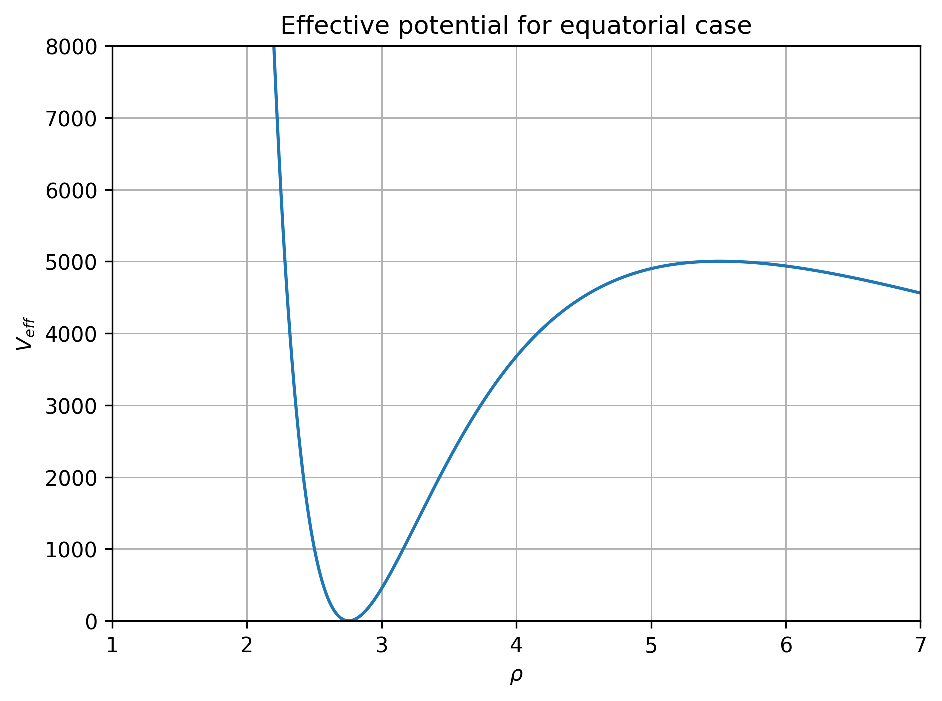
\includegraphics[scale=0.45]{Potencial_Efetivo_equatorial.pdf}
    \caption{Potencial efetivo para o caso equatorial com $c_{20} > 0$. Os pontos $\rho_1$ e $\rho_2$ correspondem ao mínimo e ao máximo locais, respectivamente. Partículas com energia total inferior a $V_{\text{eff}}(\rho_2)$ permanecem confinadas entre os pontos de retorno.}
    \label{potentEfetivo}
\end{figure}

Para verificar numericamente essas previsões, simulamos o movimento de prótons no plano equatorial usando o método de Störmer-Verlet com passo temporal $\Delta t = 0.0001$. A constante de movimento $c_{20}$ é determinada pelas condições iniciais através da equação (\ref{momentoAngular}), avaliada em $Z = 0$ (onde $R = \rho$):
\begin{equation}
    c_{20} = m\rho_0^2\dot{\phi}_0 + m\alpha_1\dfrac{1}{\rho_0}.
\end{equation}
Para o primeiro conjunto de condições iniciais, por exemplo, obtém-se $c_{20} = 1{,}844 \times 10^{-24}$ (em unidades de kg$\cdot$raios terrestres$^2\cdot$s$^{-1}$). Os três conjuntos foram escolhidos para ilustrar diferentes regimes dinâmicos:

\begin{itemize}
    \item Próton 1: $\rho(0) = 3.0$, $\dot{\rho}(0) = 10.0$, $\phi(0) = 0.0$, $\dot{\phi}(0) = 10.0$.
    \item Próton 2: $\rho(0) = 3.0$, $\dot{\rho}(0) = 80.0$, $\phi(0) = 3\pi/2$, $\dot{\phi}(0) = 10.0$.
    \item Próton 3: $\rho(0) = 3.0$, $\dot{\rho}(0) = 100.0$, $\phi(0) = \pi$, $\dot{\phi}(0) = 10.0$.
\end{itemize}

Os resultados estão apresentados na Figura \ref{agrupada}. Os prótons 1 e 2, com energia total menor do que $V_{\text{max}}$, permanecem confinados em órbitas oscilatórias ao redor da Terra. A amplitude da oscilação radial é maior para o próton 2, cuja velocidade radial inicial é mais alta. Já o próton 3, com energia cinética inicial suficiente para ultrapassar a barreira de potencial, é espalhado e escapa.

\begin{figure}[!h]
    \centering
    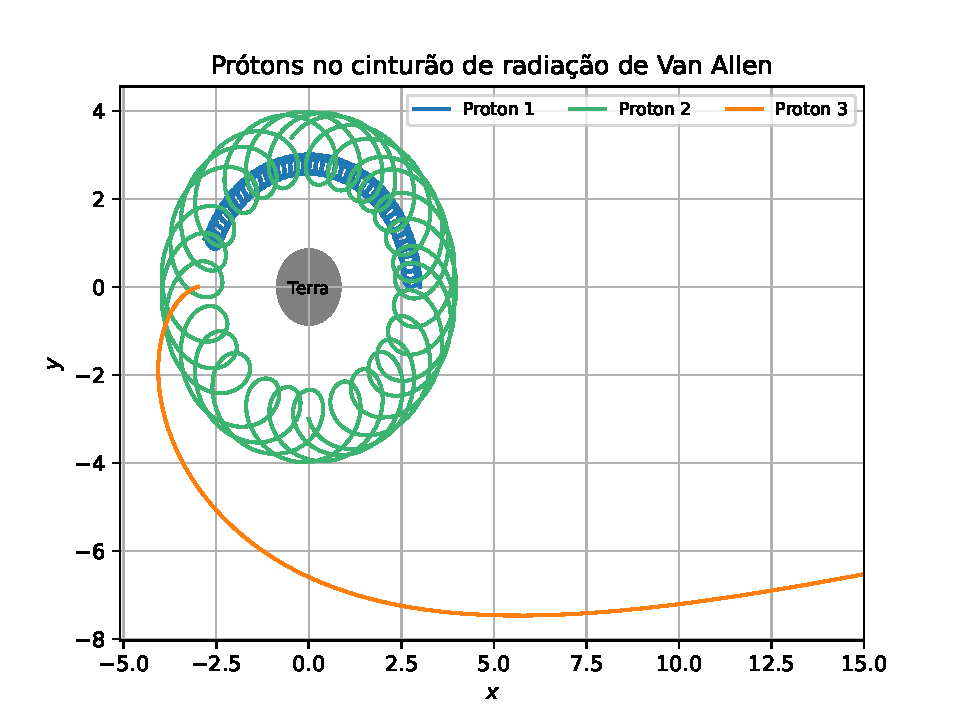
\includegraphics[scale=0.525]{plotCom3Protons.pdf}
    \caption{Trajetórias de três prótons no plano equatorial, vistas de cima (plano $xy$), com $\Delta t = 0.0001$ e $\alpha_1 = 3.04 \times 10^3$\,s$^{-1}$. Condições iniciais: Próton~1 ($\rho_0 = 3.0$, $\dot{\rho}_0 = 10.0$, $\phi_0 = 0$, $\dot{\phi}_0 = 10.0$); Próton~2 ($\rho_0 = 3.0$, $\dot{\rho}_0 = 80.0$, $\phi_0 = 3\pi/2$, $\dot{\phi}_0 = 10.0$); Próton~3 ($\rho_0 = 3.0$, $\dot{\rho}_0 = 100.0$, $\phi_0 = \pi$, $\dot{\phi}_0 = 10.0$). Os prótons 1 e 2, com energia abaixo de $V_{\text{max}}$, ficam confinados em órbitas ao redor da Terra (círculo central). O próton 3, com energia acima do limiar, escapa.}
    \label{agrupada}
\end{figure}

\subsection{Caso tridimensional}

No caso geral, as equações de movimento (\ref{eqmovimento}) devem ser resolvidas simultaneamente para $\rho(t)$ e $Z(t)$. A presença da coordenada $Z$ modifica o potencial efetivo (\ref{veff}), que agora depende de duas variáveis. A estrutura de regiões permitidas e proibidas torna-se mais complexa: as curvas de Hill no plano $(\rho, Z)$ definem faixas ao redor do equador magnético onde a partícula pode se mover.

Para a simulação tridimensional, utilizamos o método de Störmer-Verlet com passo temporal $\Delta t = 0.0002$. A constante $c_2$ é calculada a partir das condições iniciais pela equação (\ref{momentoAngular}); para o primeiro caso, obtém-se $c_2 = 1{,}776 \times 10^{-24}$. Três conjuntos de condições iniciais foram utilizados:

\begin{itemize}
    \item Próton 1: $\rho(0) = 3.0$, $\dot{\rho}(0) = 10.0$, $\phi(0) = 0.0$, $\dot{\phi}(0) = 10.0$, $Z(0) = 0.5$, $\dot{Z}(0) = 0.0$.
    \item Próton 2: $\rho(0) = 3.0$, $\dot{\rho}(0) = 80.0$, $\phi(0) = \pi$, $\dot{\phi}(0) = 10.0$, $Z(0) = 0.5$, $\dot{Z}(0) = 0.0$.
    \item Próton 3: $\rho(0) = 3.0$, $\dot{\rho}(0) = 100.0$, $\phi(0) = 5.26$, $\dot{\phi}(0) = 10.0$, $Z(0) = 0.5$, $\dot{Z}(0) = 0.0$.
\end{itemize}

A Figura \ref{resultado3Protons2DGeral} mostra as trajetórias resultantes projetadas no plano meridional $(\rho, Z)$ e em perspectiva tridimensional. Ao contrário do caso equatorial, onde a trajetória confinada é periódica, no caso tridimensional a partícula oscila simultaneamente na direção radial e na direção $Z$, percorrendo a região toroidal em torno da Terra sem repetir a mesma trajetória. A partícula permanece confinada pela barreira de potencial, mas sua trajetória no plano meridional preenche densamente a região acessível. A depender das condições iniciais, a órbita pode ser quase-periódica ou caótica, uma consequência direta da não integrabilidade do sistema.

\begin{figure}[!h]
    \centering
    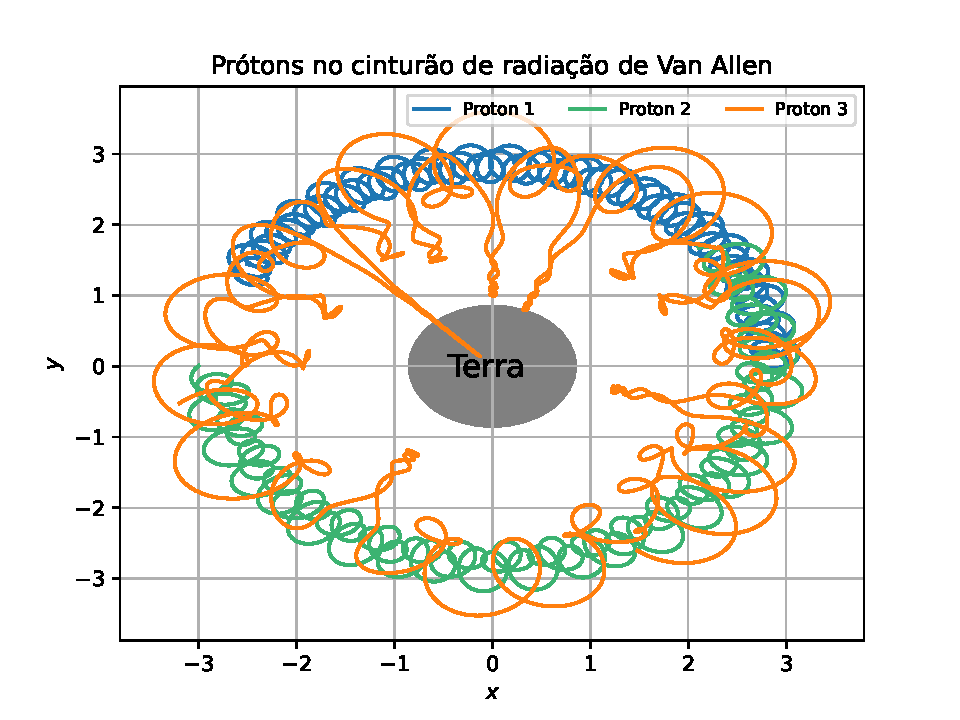
\includegraphics[scale=0.525]{plot3DPlano2.pdf}
    \caption{Trajetórias de três prótons no caso tridimensional, com $\Delta t = 0.0002$ e $\alpha_1 = 3.04 \times 10^3$\,s$^{-1}$. Condições iniciais: Próton~1 ($\rho_0 = 3.0$, $\dot{\rho}_0 = 10.0$, $\phi_0 = 0$, $\dot{\phi}_0 = 10.0$, $Z_0 = 0.5$, $\dot{Z}_0 = 0$); Próton~2 ($\rho_0 = 3.0$, $\dot{\rho}_0 = 80.0$, $\phi_0 = \pi$, $\dot{\phi}_0 = 10.0$, $Z_0 = 0.5$, $\dot{Z}_0 = 0$); Próton~3 ($\rho_0 = 3.0$, $\dot{\rho}_0 = 100.0$, $\phi_0 = 5.26$, $\dot{\phi}_0 = 10.0$, $Z_0 = 0.5$, $\dot{Z}_0 = 0$). As projeções no plano meridional mostram que as partículas confinadas oscilam tanto radialmente quanto na direção $Z$, preenchendo a região permitida. A estrutura toroidal resultante é uma idealização do cinturão de radiação de Van Allen.}
    \label{resultado3Protons2DGeral}
\end{figure}

A região toroidal onde as partículas permanecem confinadas corresponde, em nosso modelo simplificado, ao cinturão de radiação de Van Allen. Na natureza, o cinturão de Van Allen é formado por prótons e elétrons de diferentes energias, e sua estrutura detalhada depende de efeitos que não foram incluídos neste modelo, como variações temporais do campo geomagnético, interações com o vento solar e efeitos relativísticos. Ainda assim, o modelo dipolar reproduz corretamente o mecanismo básico de confinamento magnético.

Vale notar que, durante a oscilação latitudinal, a trajetória da partícula confinada pode atingir a superfície terrestre (representada pela esfera de raio $R = 1$ em nossas unidades). Partículas que chegam a altitudes suficientemente baixas interagem com a atmosfera, depositam energia e produzem emissões luminosas: as auroras polares. Esse fenômeno ocorre preferencialmente em latitudes altas, onde as linhas de campo convergem. Uma modelagem mais detalhada exigiria efeitos atmosféricos e, possivelmente, uma formulação vinculada à superfície terrestre, como a que apresentamos a seguir.

\subsection{Caso vinculado: movimento sobre uma superfície esférica}

O problema de Störmer na forma livre, discutido nas seções anteriores, é não integrável. Existe, porém, uma variante do problema que admite tratamento analítico: o caso em que a partícula carregada é restrita a se mover sobre uma superfície esférica de raio $R_s$ centrada no dipolo magnético \cite{StormerEsferico, PinaCortesElliptic}. Essa formulação, proposta por Cortés e Cortés Poza \cite{StormerEsferico}, modela de forma simplificada a interação de partículas carregadas com a atmosfera terrestre em altitudes fixas. O interesse teórico dessa formulação é que o vínculo holonômico torna integrável um sistema que, sem ele, não o é.

\subsubsection{Formulação sobre a esfera}

Com a partícula restrita à esfera $R = R_s$, restam dois graus de liberdade: o ângulo polar $\theta$ (medido a partir do polo norte) e o ângulo azimutal $\varphi$. O potencial vetor do dipolo magnético, restrito à superfície, tem apenas componente azimutal:

\begin{equation}\label{Asfera}
    \boldsymbol{A} = -\dfrac{\mu_0 \mu \sin\theta}{4\pi R_s^2}\,\boldsymbol{e}_\varphi,
\end{equation}

\noindent onde $\mu$ é o módulo do momento de dipolo magnético, o mesmo que aparece na definição de $M_z$ na equação (\ref{potencialVetor}). A lagrangiana do sistema é

\begin{equation}\label{lagSfera}
    L = \dfrac{1}{2}MR_s^2\left(\dot{\theta}^2 + \dot{\varphi}^2\sin^2\theta\right) - k_s\dot{\varphi}\sin^2\theta,
\end{equation}

\noindent onde $M$ é a massa da partícula e $k_s = q\mu_0 \mu/(4\pi R_s)$ é uma constante com dimensão de momento angular que condensa as propriedades do dipolo e da partícula. O último termo acopla o campo magnético ao movimento azimutal.

Como no caso livre, a coordenada $\varphi$ é cíclica, e o momento canônico conjugado

\begin{equation}\label{pphiSfera}
    p_\varphi = MR_s^2\dot{\varphi}\sin^2\theta - k_s\sin^2\theta
\end{equation}

\noindent é uma constante de movimento. A hamiltoniana coincide com a energia cinética (a força magnética não realiza trabalho) e fornece a segunda constante de movimento. Com dois graus de liberdade e duas constantes de movimento independentes, o sistema é integrável no sentido de Liouville \cite{Saletan}.

\subsubsection{Potencial efetivo e regimes de movimento}

A hamiltoniana pode ser escrita como

\begin{equation}\label{hamSfera}
    H = \dfrac{1}{2MR_s^2}\left[p_\theta^2 + \dfrac{\left(p_\varphi + k_s\sin^2\theta\right)^2}{\sin^2\theta}\right] = \dfrac{p_\theta^2}{2MR_s^2} + V_{\text{eff}}(\theta),
\end{equation}

\noindent onde o potencial efetivo é

\begin{equation}\label{veffSfera}
    V_{\text{eff}}(\theta) = \dfrac{1}{2MR_s^2}\dfrac{\left(p_\varphi + k_s\sin^2\theta\right)^2}{\sin^2\theta}.
\end{equation}

A estrutura desse potencial depende da relação entre $|p_\varphi|$ e $k_s$. Quando $|p_\varphi| < k_s$, o potencial exibe dois poços separados por uma barreira no equador ($\theta = \pi/2$), formando um potencial biestável. Nesse regime, a partícula pode ficar confinada em um dos hemisférios, oscilando entre dois ângulos de retorno em $\theta$ sem cruzar o equador. Quando $|p_\varphi| \geq k_s$, a barreira desaparece e a partícula oscila entre os dois hemisférios.

Os polos ($\theta = 0$ e $\theta = \pi$) são sempre repulsivos, pois $V_{\text{eff}} \to \infty$ quando $\theta \to 0$ ou $\pi$ (devido ao fator $\csc^2\theta$). A partícula jamais atinge os polos com energia finita.

\subsubsection{Solução analítica e validação numérica}

Com a mudança de variável $z = \cos\theta$, a equação de movimento para $\theta$ se reduz à equação de um oscilador em um potencial quártico \cite{PinaCortesElliptic}:

\begin{equation}\label{quartico}
    \dot{z}^2 = -b^2(z^2 - A)(z^2 - B),
\end{equation}

\noindent onde $A$ e $B$ são constantes que dependem dos parâmetros adimensionais $a = p_\varphi/\ell$ e $b = k_s/\ell$, com $\ell = \sqrt{2MR_s^2 K}$ sendo o momento angular característico e $K$ a energia cinética (constante). Piña e Cortés \cite{PinaCortesElliptic} demonstraram que a solução dessa equação se expressa em termos das funções elípticas de Jacobi:

\begin{equation}\label{solucaoJacobi}
    z(\tau) = \begin{cases}
        \sqrt{B}\,\text{dn}(b\sqrt{B}\,\tau,\,\kappa) & \text{se } A > 0 \text{ (um hemisfério)}\\[6pt]
        \sqrt{B}\,\text{cn}(b\sqrt{B-A}\,\tau,\,\kappa) & \text{se } A < 0 \text{ (dois hemisférios)}
    \end{cases}
\end{equation}

\noindent onde $\tau$ é o tempo adimensional, $\text{dn}$ e $\text{cn}$ são funções elípticas de Jacobi, e $\kappa$ é o módulo elíptico, determinado por $A$ e $B$.

Essa solução analítica permite validar diretamente o integrador de Störmer-Verlet. Utilizando os mesmos parâmetros do artigo original ($M = 2$, $R_s = 10$, $k_s = 0.5$, em unidades arbitrárias), simulamos numericamente o movimento da partícula sobre a esfera e comparamos as trajetórias com a solução elíptica exata. As Figuras \ref{fig:esfera_banda}--\ref{fig:esfera_loops} mostram essa comparação para três casos representativos que cobrem os diferentes regimes do potencial efetivo (\ref{veffSfera}):

\begin{itemize}
    \item \textbf{Banda no hemisfério norte} ($\theta_0 = \pi/3$, $p_{\theta 0} = 0$, $p_\varphi = 0.394$): a partícula oscila em $\theta$ dentro de uma faixa estreita no hemisfério norte, traçando uma banda sobre a esfera. Regime $A > 0$, solução via $\text{dn}$.
    \item \textbf{Cruza o equador} ($\theta_0 = 0.6$ rad, $p_{\theta 0} = 0.2525$, $p_\varphi = 0.25$): a partícula possui energia suficiente para cruzar a barreira equatorial do potencial biestável e percorre ambos os hemisférios. Regime $A < 0$, solução via $\text{cn}$.
    \item \textbf{Laços} ($\theta_0 = \pi/4$, $p_{\theta 0} = 0.3$, $p_\varphi = -0.15$): quando $-k_s < p_\varphi < 0$, a trajetória exibe laços que não envolvem nenhum dos polos \cite{StormerEsferico}. Regime $A > 0$, solução via $\text{dn}$.
\end{itemize}

Em cada figura, o painel superior sobrepõe as trajetórias do integrador numérico (azul) e da solução analítica (vermelho) sobre a esfera. O painel inferior mostra o erro de posição normalizado $\|\mathbf{r}_{\text{SV}}(t) - \mathbf{r}_{\text{an}}(t)\| / R_s$ ao longo da simulação. Nos três casos, esse erro oscila periodicamente na faixa de $10^{-8}$ a $10^{-7}$, sem crescimento secular. O erro relativo de energia, por sua vez, permanece no nível da precisão aritmética de ponto flutuante ($\sim 10^{-15}$). Esse comportamento é esperado de um integrador simplético (Seção \ref{sec:simplectico}): conforme a análise de erro retroativo \cite{stormer-verlet, Hairer2003}, o Störmer-Verlet resolve exatamente uma hamiltoniana modificada $\widetilde{H} = H + \mathcal{O}(\Delta t^2)$. A órbita numérica segue, portanto, uma trajetória fisicamente consistente, ligeiramente deslocada da original, mas sem acúmulo de erro.

\begin{figure}[!h]
    \centering
    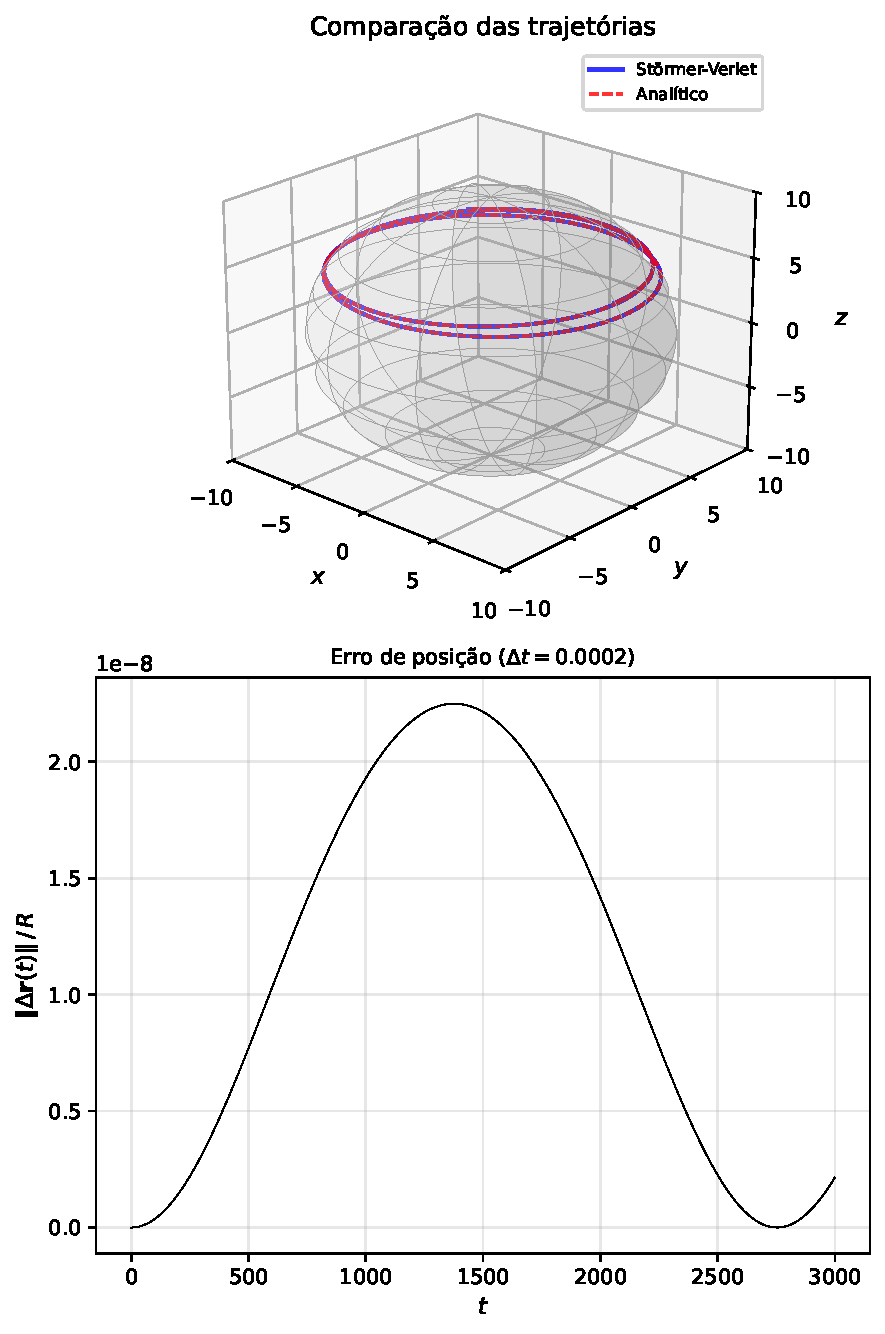
\includegraphics[scale=0.45]{validation_sphere_banda.pdf}
    \caption{Validação: caso banda no hemisfério norte ($\theta_0 = \pi/3$, $p_{\theta 0} = 0$, $p_\varphi = 0.394$, $t = 3000$, $1{,}5 \times 10^7$ passos). Acima: trajetórias sobre a esfera (azul: Störmer-Verlet, vermelho: analítico). Abaixo: erro de posição normalizado $\|\mathbf{r}_{\text{SV}} - \mathbf{r}_{\text{an}}\|/R_s$.}
    \label{fig:esfera_banda}
\end{figure}

\begin{figure}[!h]
    \centering
    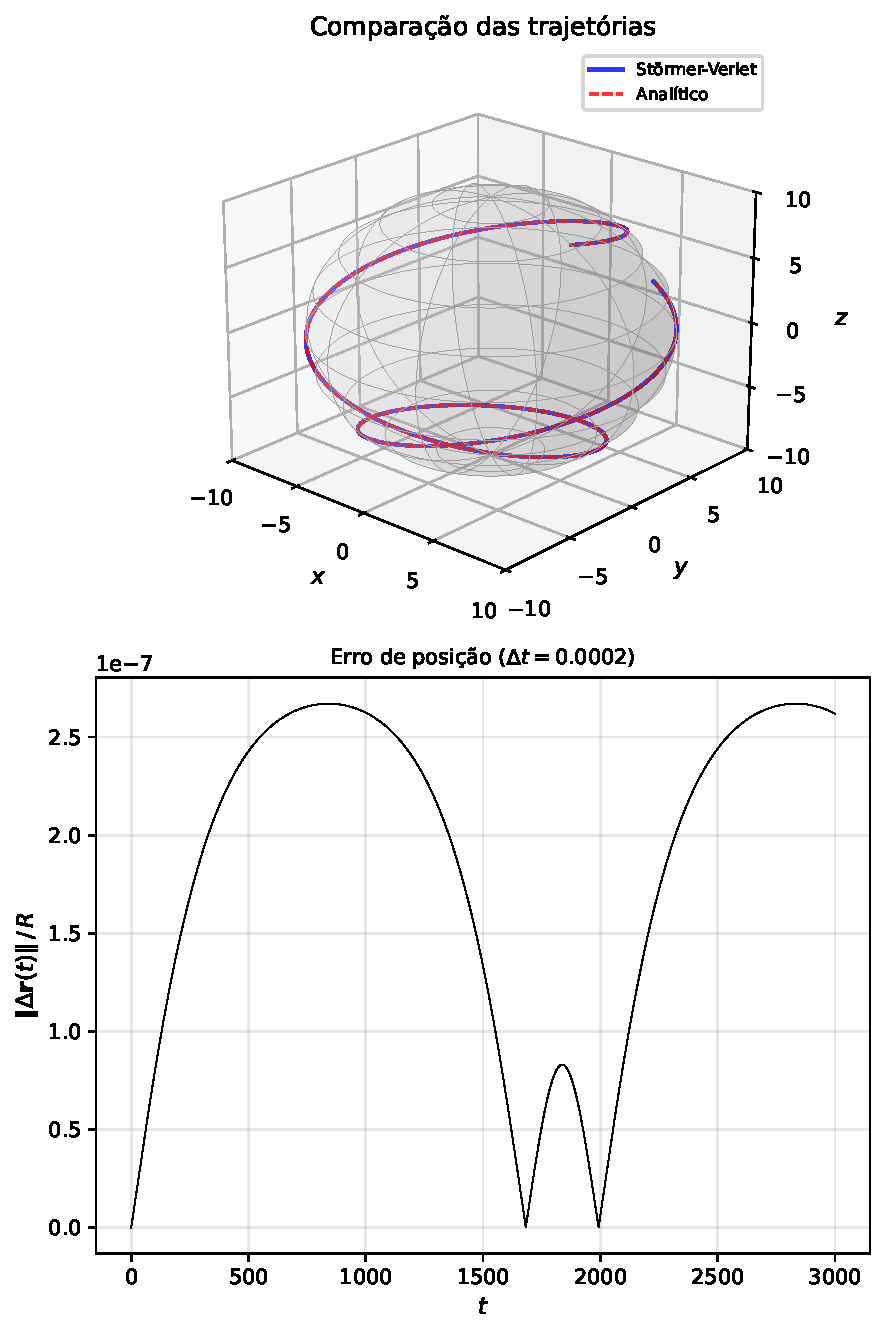
\includegraphics[scale=0.45]{validation_sphere_equador.pdf}
    \caption{Validação: caso travessia do equador ($\theta_0 = 0.6$ rad, $p_{\theta 0} = 0.2525$, $p_\varphi = 0.25$, $t = 3000$, $1{,}5 \times 10^7$ passos). A partícula cruza a barreira equatorial do potencial biestável e percorre ambos os hemisférios.}
    \label{fig:esfera_equador}
\end{figure}

\begin{figure}[!h]
    \centering
    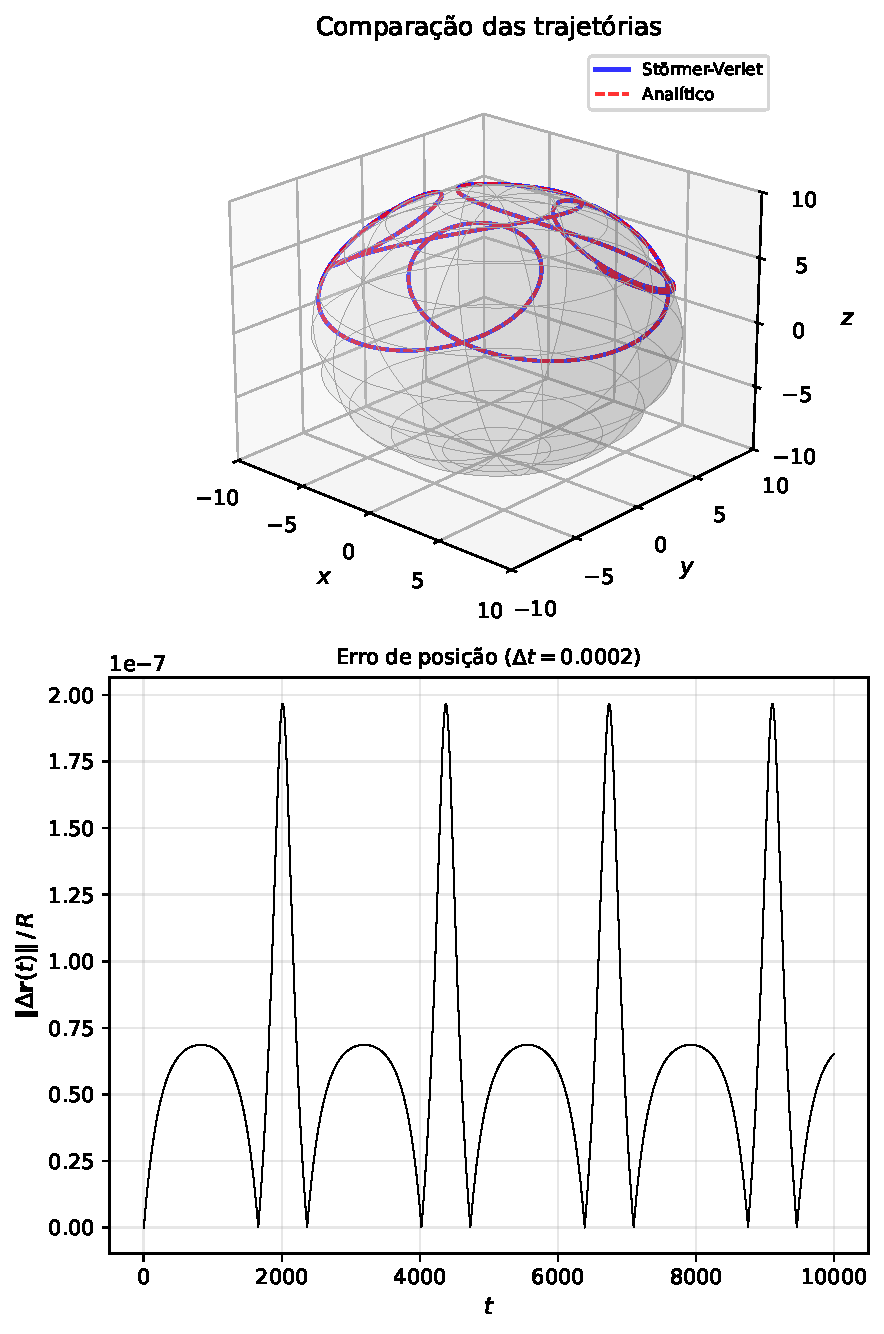
\includegraphics[scale=0.45]{validation_sphere_loops.pdf}
    \caption{Validação: caso laços ($\theta_0 = \pi/4$, $p_{\theta 0} = 0.3$, $p_\varphi = -0.15$, $t = 10000$, $5 \times 10^7$ passos). Quando $-k_s < p_\varphi < 0$, a trajetória exibe laços que não envolvem nenhum dos polos \cite{StormerEsferico}.}
    \label{fig:esfera_loops}
\end{figure}

A existência dessa solução analítica revela ainda uma conexão entre o problema de Störmer e a dinâmica de corpos rígidos. Piña e Cortés \cite{PinaCortesElliptic} mostraram que as soluções em termos de $\text{dn}$ e $\text{cn}$ têm a mesma estrutura matemática das soluções do pião de Euler (rotação livre de um corpo rígido assimétrico) e do pião de Lagrange (corpo rígido simétrico com gravidade). Essa correspondência não é acidental: em ambos os problemas, as equações de movimento se reduzem a uma equação diferencial com potencial quártico em $z = \cos\theta$, cuja solução é dada pelas mesmas classes de funções elípticas. O problema de Störmer sobre a esfera pode, assim, servir como porta de entrada para as funções elípticas de Jacobi e para a dinâmica de corpos rígidos a partir de um contexto eletromagnético.

\section{Conclusões}

O problema de Störmer reúne, num mesmo sistema, tópicos que os cursos de graduação costumam tratar em separado: a formulação lagrangiana e hamiltoniana, constantes de movimento, potencial efetivo, integração numérica de sistemas dinâmicos e, no caso vinculado à esfera, funções especiais. Neste artigo, percorremos essas etapas da derivação analítica à simulação com o integrador simplético de Störmer-Verlet, incluindo a validação do método numérico contra uma solução exata.

A análise do caso equatorial mostrou como o potencial efetivo controla o confinamento radial: partículas com energia abaixo do máximo do potencial ficam presas em órbitas oscilatórias, enquanto partículas com energia acima desse limiar escapam. As simulações confirmaram esse critério e permitiram visualizar os dois regimes.

O caso tridimensional acrescentou a oscilação latitudinal, e as simulações mostraram a formação de trajetórias confinadas em uma região toroidal ao redor da Terra, o que corresponde, em nosso modelo idealizado, ao cinturão de radiação de Van Allen. A sensibilidade às condições iniciais, característica da não integrabilidade do sistema, abre espaço para investigações sobre o caráter caótico das trajetórias, cuja caracterização mais precisa, via seções de Poincaré ou expoentes de Lyapunov, fica como proposta para um trabalho futuro.

O caso vinculado à esfera mostrou como a imposição de um vínculo holonômico transforma o sistema não integrável em um sistema integrável, com solução analítica em funções elípticas de Jacobi. A comparação direta entre a solução analítica e a integração numérica pelo método de Störmer-Verlet validou o integrador: ao longo de simulações com até $5 \times 10^7$ passos temporais, o erro de posição permaneceu na faixa de $10^{-8}$ a $10^{-7}$ do raio da esfera, sem crescimento secular.

O código-fonte das simulações, tanto para o caso livre quanto para o caso esférico, foi implementado em linguagem C e está disponível em repositório público.\footnote{\url{https://github.com/Shnrqpdr/Stormer-Problem}}

\section*{Declaração de financiamento}

Este trabalho foi desenvolvido no âmbito do Programa Institucional de Bolsas de Iniciação Científica (PIBIC) da Universidade Federal Fluminense, com bolsa financiada pelo CNPq.

\section*{Declaração de disponibilidade de dados}

Todo o conjunto de dados que dá suporte aos resultados deste estudo foi publicado no próprio artigo.

\begin{thebibliography}{99}

\bibitem{Birkeland} K. Birkeland, \textit{The Norwegian Aurora Polaris Expedition 1902--1903} (H. Aschehoug \& Co., Christiania, 1908).

\bibitem{Stormer} C. Störmer, Periodische Elektronenbahnen im Felde eines Elementarmagneten und ihre Anwendung auf Brüches Modellversuche und auf Eschenhagens Elementarwellen des Erdmagnetismus, Zeitschrift für Astrophysik \textbf{1}, 237 (1930).

\bibitem{Stormer2} C. Störmer, Twenty-five years' work on the polar aurora, Terrestrial Magnetism and Atmospheric Electricity \textbf{35}, 193 (1930).

\bibitem{Stormer3} C. Störmer, \textit{The Polar Aurora} (Clarendon Press, Oxford, 1955).

\bibitem{Clay} J. Clay e H.P. Berlage, Die Intensität der Höhenstrahlung in verschiedenen Breiten und die Erklärung des Breiteneffektes, Naturwissenschaften \textbf{20}, 687 (1932).

\bibitem{Compton} A.H. Compton, Variation of the cosmic rays with latitude, Physical Review \textbf{41}, 111 (1932).

\bibitem{VanAllen} J.A. Van Allen e L.A. Frank, Radiation around the Earth to a radial distance of 107,400 km, Nature \textbf{183}, 430 (1959).

\bibitem{atlantico} C.I. Underwood, D.J. Brock, P.S. Williams, S. Kim, R. Dilão, P. Ribeiro Santos, M.C. Brito, C.S. Dyer e A.J. Sims, Radiation environment measurements with the cosmic ray experiments on-board the KITSAT-1 and PoSAT-1 micro-satellites, IEEE Transactions on Nuclear Science \textbf{41}, 2353 (1994).

\bibitem{ESA} E.J. Daly, The evaluation of space radiation environments for ESA projects, ESA Bulletin \textbf{12}, 229 (1988).

\bibitem{Stassinopoulos} E.G. Stassinopoulos e J.P. Raymond, The space radiation environment for electronics, Proceedings of the IEEE \textbf{76}, 1423 (1988).

\bibitem{ruidilao} R. Dilão e R. Alves-Pires, Chaos in the Störmer problem, em: \textit{Differential Equations, Chaos and Variational Problems}, editado por V. Staicu (Springer, Basel, 2007), p. 175--194.

\bibitem{stormer-verlet} E. Hairer, C. Lubich e G. Wanner, \textit{Geometric Numerical Integration: Structure-Preserving Algorithms for Ordinary Differential Equations} (Springer, Berlin, 2006).

\bibitem{Goldstein} H. Goldstein, C. Poole e J. Safko, \textit{Classical Mechanics} (Addison-Wesley, San Francisco, 2002), 3ª ed.

\bibitem{StormerEsferico} E. Cortés e D. Cortés Poza, Störmer problem restricted to a spherical surface, European Journal of Physics \textbf{36}, 055009 (2015).

\bibitem{PinaCortesElliptic} E. Piña e E. Cortés, Störmer problem restricted to a spherical surface and the Euler and Lagrange tops, European Journal of Physics \textbf{37}, 065009 (2016).

\bibitem{Taylor} J.R. Taylor, \textit{Classical Mechanics} (University Science Books, Sausalito, 2005).

\bibitem{Saletan} J.V. José e E.J. Saletan, \textit{Classical Dynamics: A Contemporary Approach} (Cambridge University Press, Cambridge, 1998).

\bibitem{Newton} I. Newton, \textit{Philosophiæ Naturalis Principia Mathematica} (Royal Society, Londres, 1687).

\bibitem{Verlet} L. Verlet, Computer ``experiments'' on classical fluids. I. Thermodynamical properties of Lennard-Jones molecules, Physical Review \textbf{159}, 98 (1967).

\bibitem{Hairer2003} E. Hairer, C. Lubich e G. Wanner, Geometric numerical integration illustrated by the Störmer--Verlet method, Acta Numerica \textbf{12}, 399 (2003).

\end{thebibliography}

\end{document}
